\section[Performance of the charged-particle-tracking system]{Performance of the charged-particle-tracking system \label{sec:trackingperformance}}
\subsection{Track reconstruction}

The first stage in track reconstruction is pattern recognition.  Hits in adjacent
 layers in the FDC in each package are formed into track segments that are 
linked together with other segments in other packages to form FDC track 
candidates using a helical model for the track parameters.
Hits in adjacent rings in the axial layers of the CDC are also associated into 
segments that are linked together with other segments in other axial layers
and fitted with circles in the projection perpendicular to the beam line. Intersections between these circles and the stereo wires are found and a linear fit is performed to find a $z-$position near the beamline and the tangent to the dip
 angle $\lambda=\pi/2-\theta$.  These parameters, in addition to the circle fit 
parameters, form a CDC track candidate for each set of linked axial and stereo 
layers. Candidates that emerge from the target, and pass through both FDC and CDC in the  $5^\circ-20^\circ$ range, are linked together.

The second stage uses a Kalman filter \cite{KalmanFilter, KalmanFilter2} to find the fitted track parameters
\{z,D,$\phi$,$\tan\lambda$,$q/p_T$\}
at the position of closest approach of the track to the beam line using the 
track candidate parameters as an initial guess, where $D$ is the signed 
distance of closest approach to the beam line.  The Kalman filter proceeds in 
steps from
the hits farthest from the beam line toward the beam line, taking into account
energy loss and multiple scattering at each step along the way, according to a
map of the magnetic field within the bore of the solenoid magnet.  For the 
first initial pass of the filter, the drift time information from the 
wires is note used.  Each particle is assumed to be a pion, except for low momentum track 
candidates ($p<0.8$~GeV/$c$), for which the fits are performed with a proton hypothesis.

The third stage matches each fitted track from the second 
stage to either the Start Counter, the Time-of-Flight scintillators, the Barrel Calorimeter, or the 
Forward Calorimeter to determine a start time $t_0$ so that the drift time to each wire 
associated with the track can be used in the fit.  Each track is refitted with
the drift information, separately for each value of mass for particles in the set \{$e^\pm,\pi^\pm,K^\pm,p^\pm$\}.




\subsection{Momentum resolution}

The momentum resolution as a function of angle and magnitude for pions and 
protons is shown in Fig.~\ref{fig:dp_p}.  The angular resolution is shown in 
Fig.~\ref{fig:angle res}.


\begin{figure}[tbp]
\begin{center}
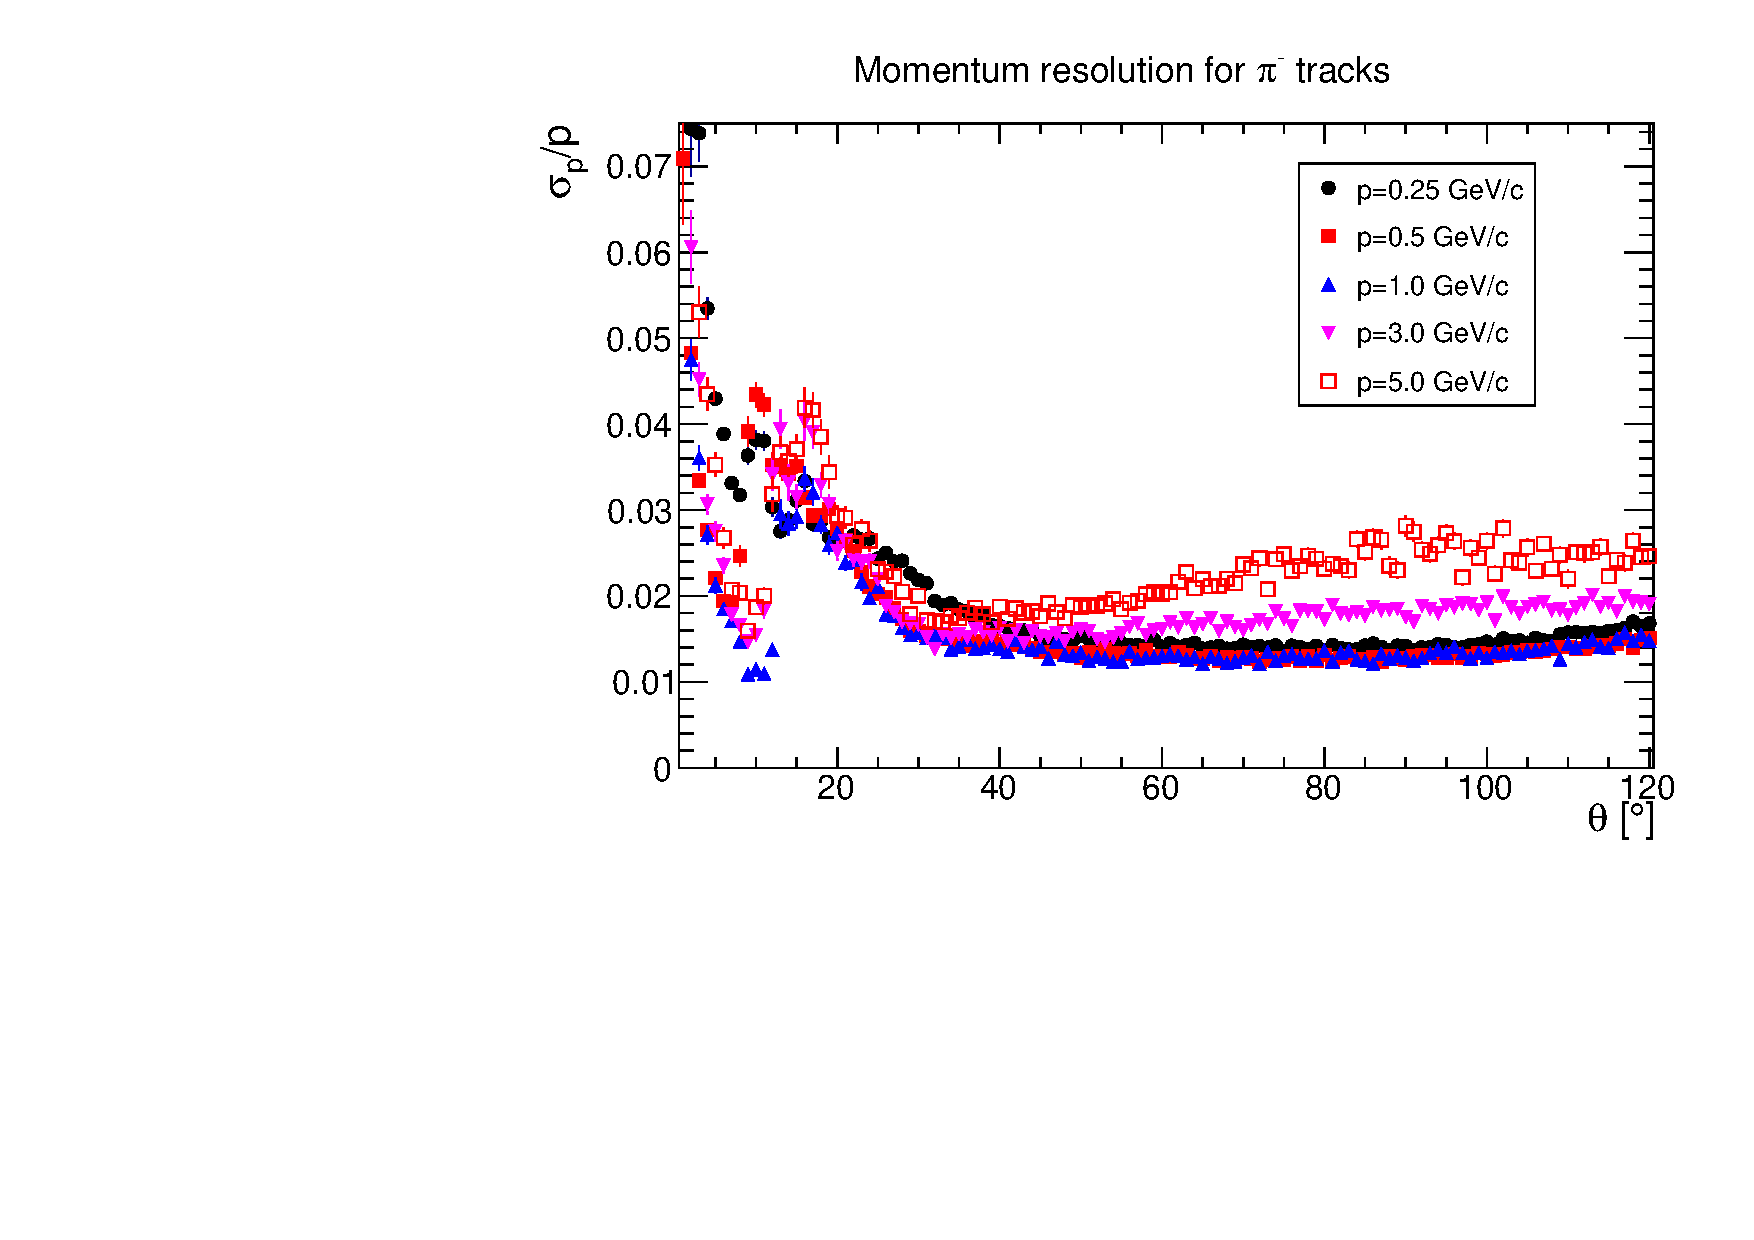
\includegraphics[width=0.45\textwidth]{figures/PionMomentumResolution.pdf}
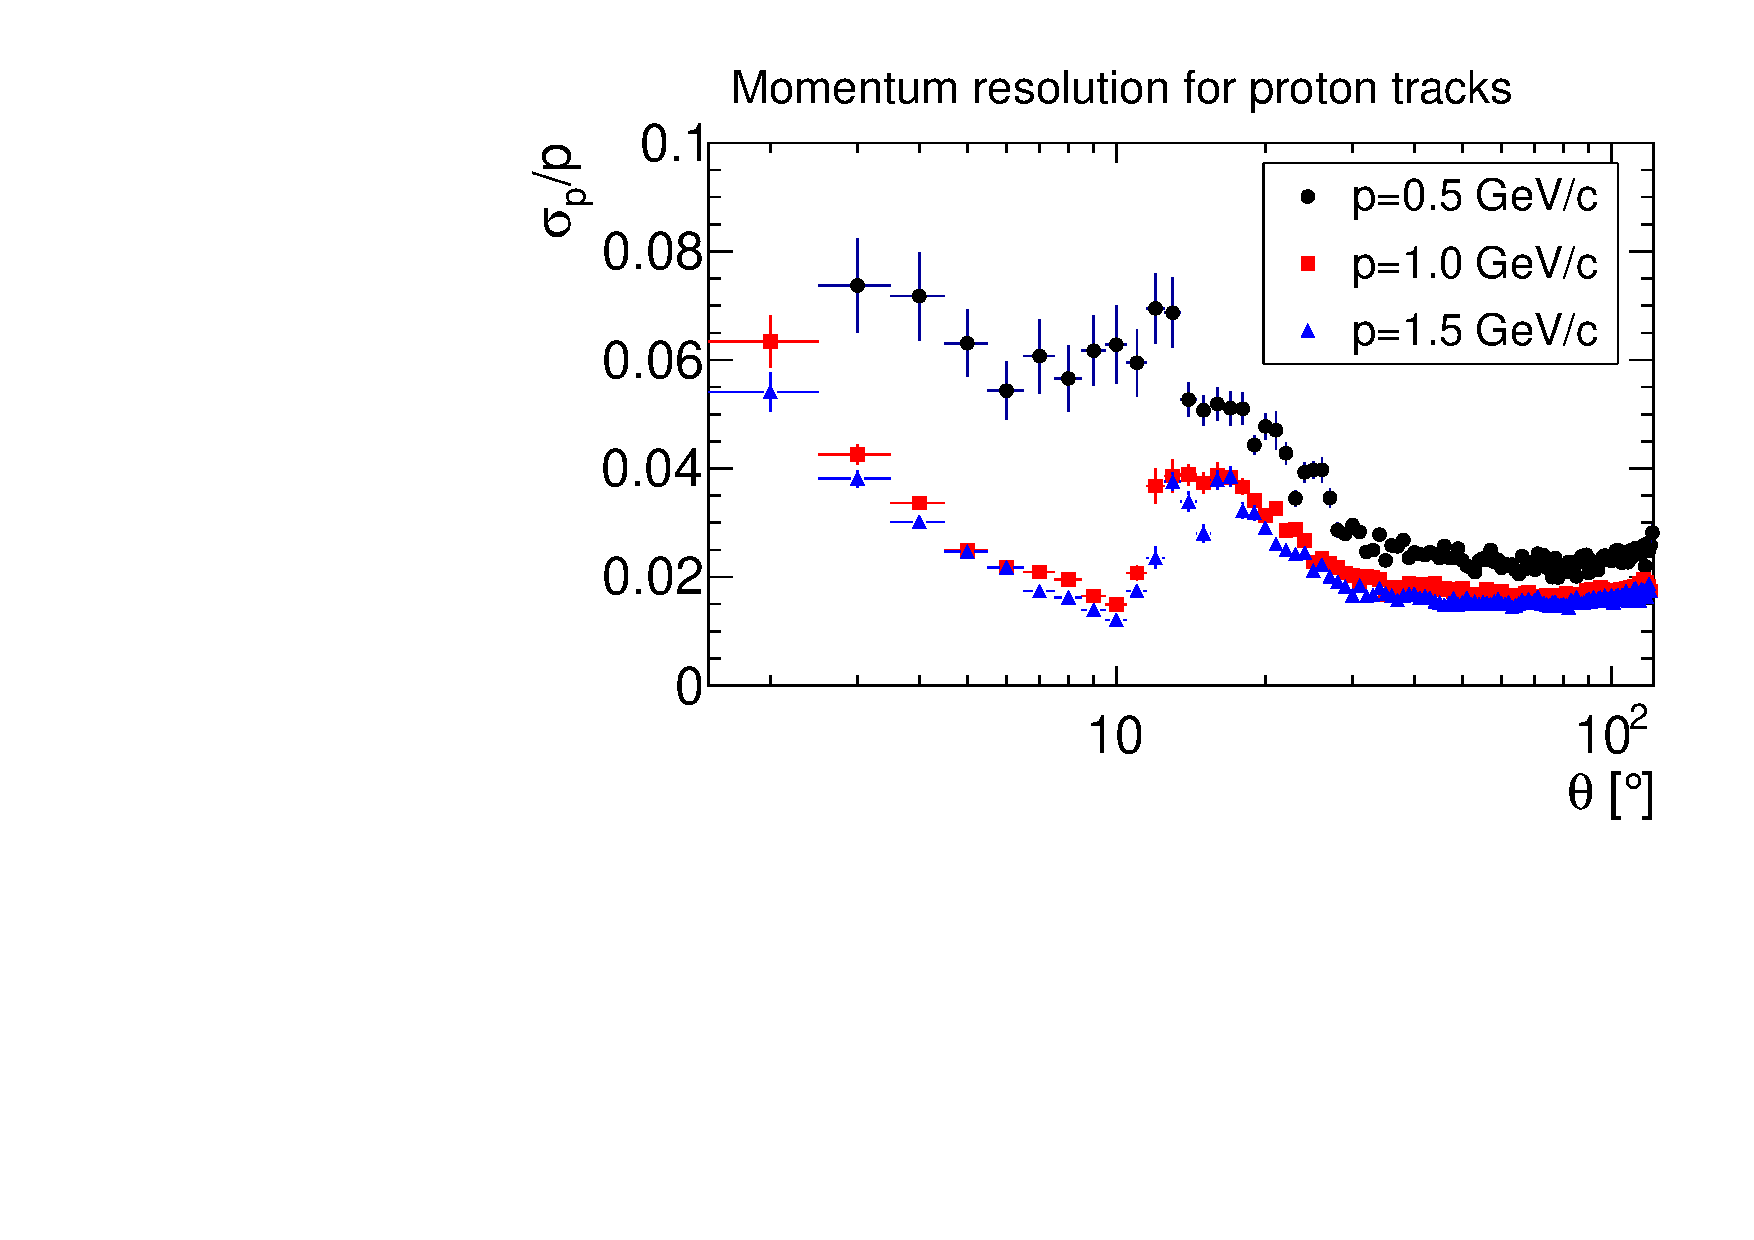
\includegraphics[width=0.45\textwidth]{figures/ProtonMomentumResolution.pdf}
\caption{\label{fig:dp_p} (Left) Momentum resolution for $\pi^-$ tracks.
(Right) Momentum resolution for proton tracks.}
\end{center}
\end{figure}

\begin{figure}[tbp]
\begin{center}
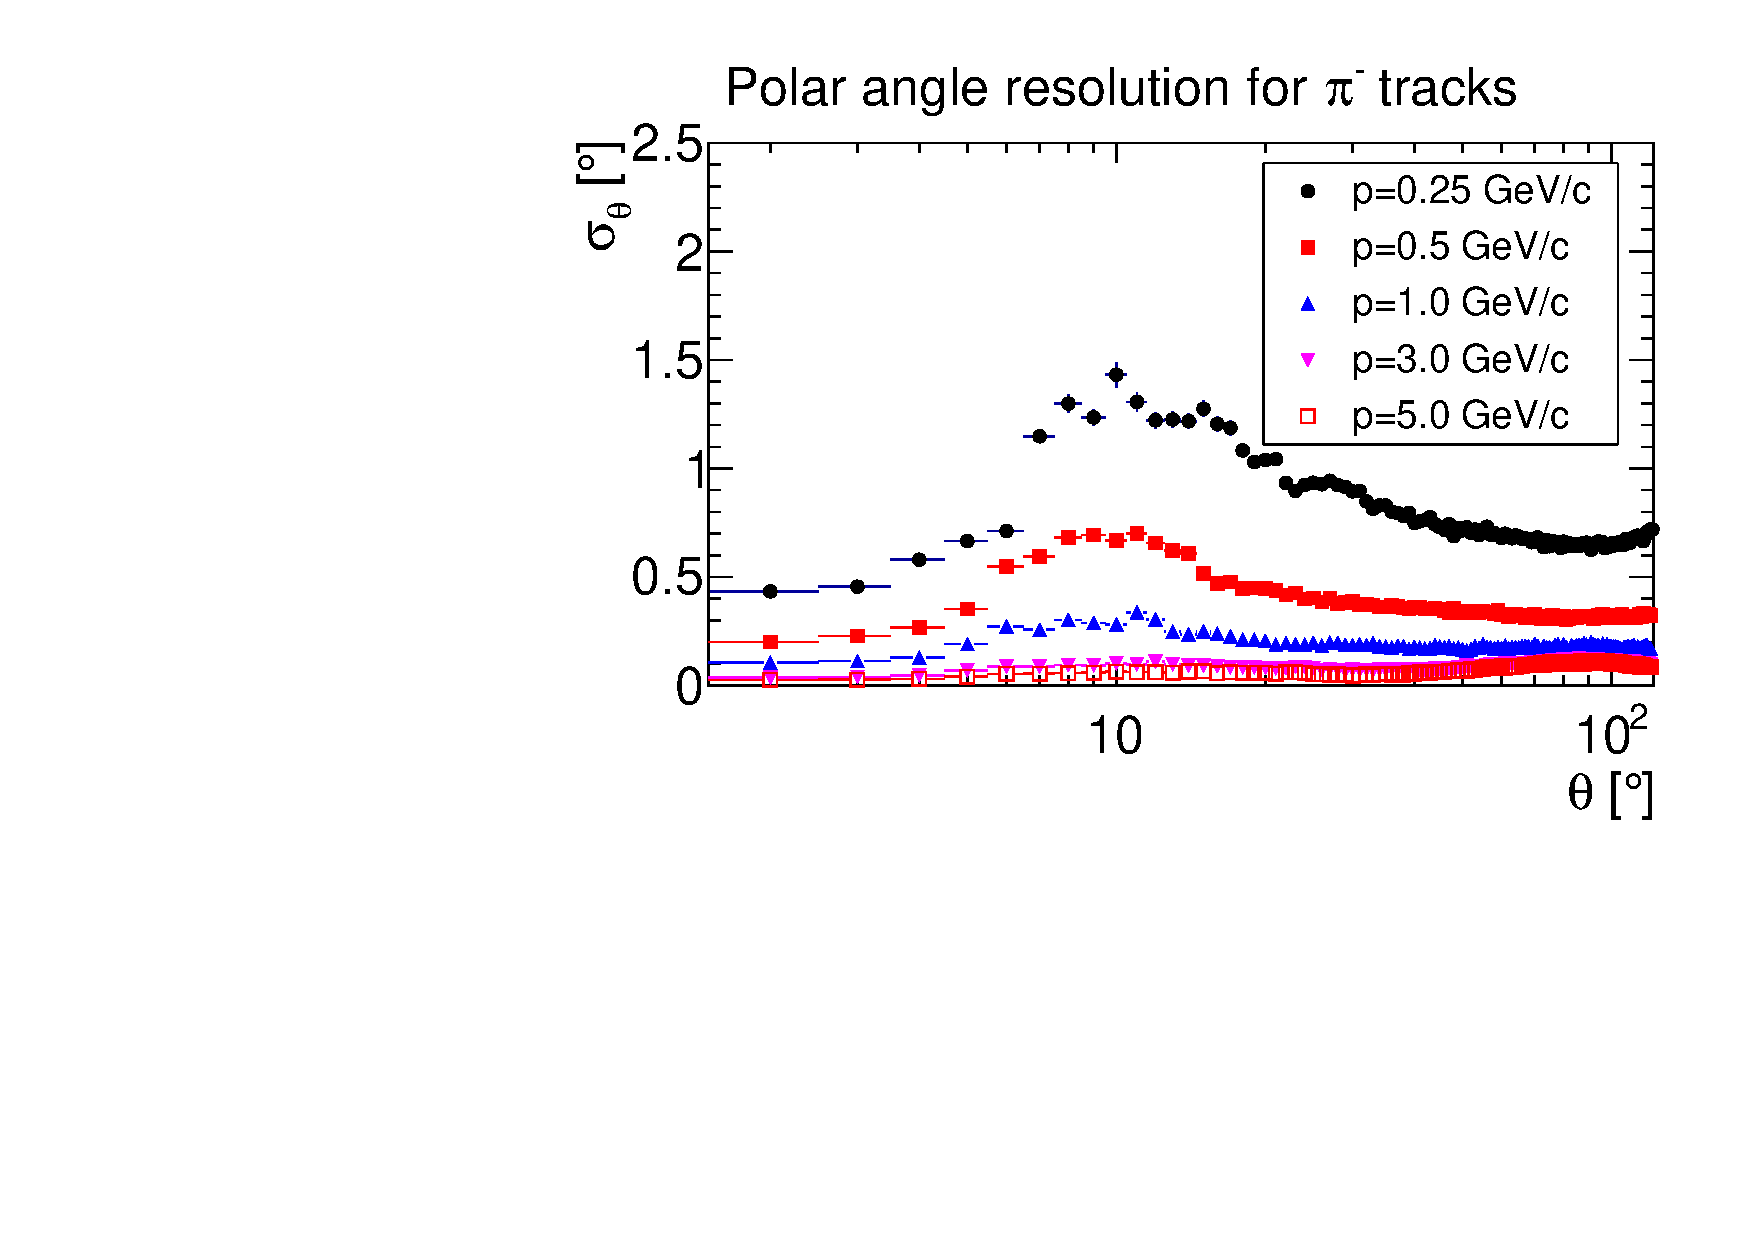
\includegraphics[width=0.45\textwidth]{figures/PionThetaResolution.pdf}
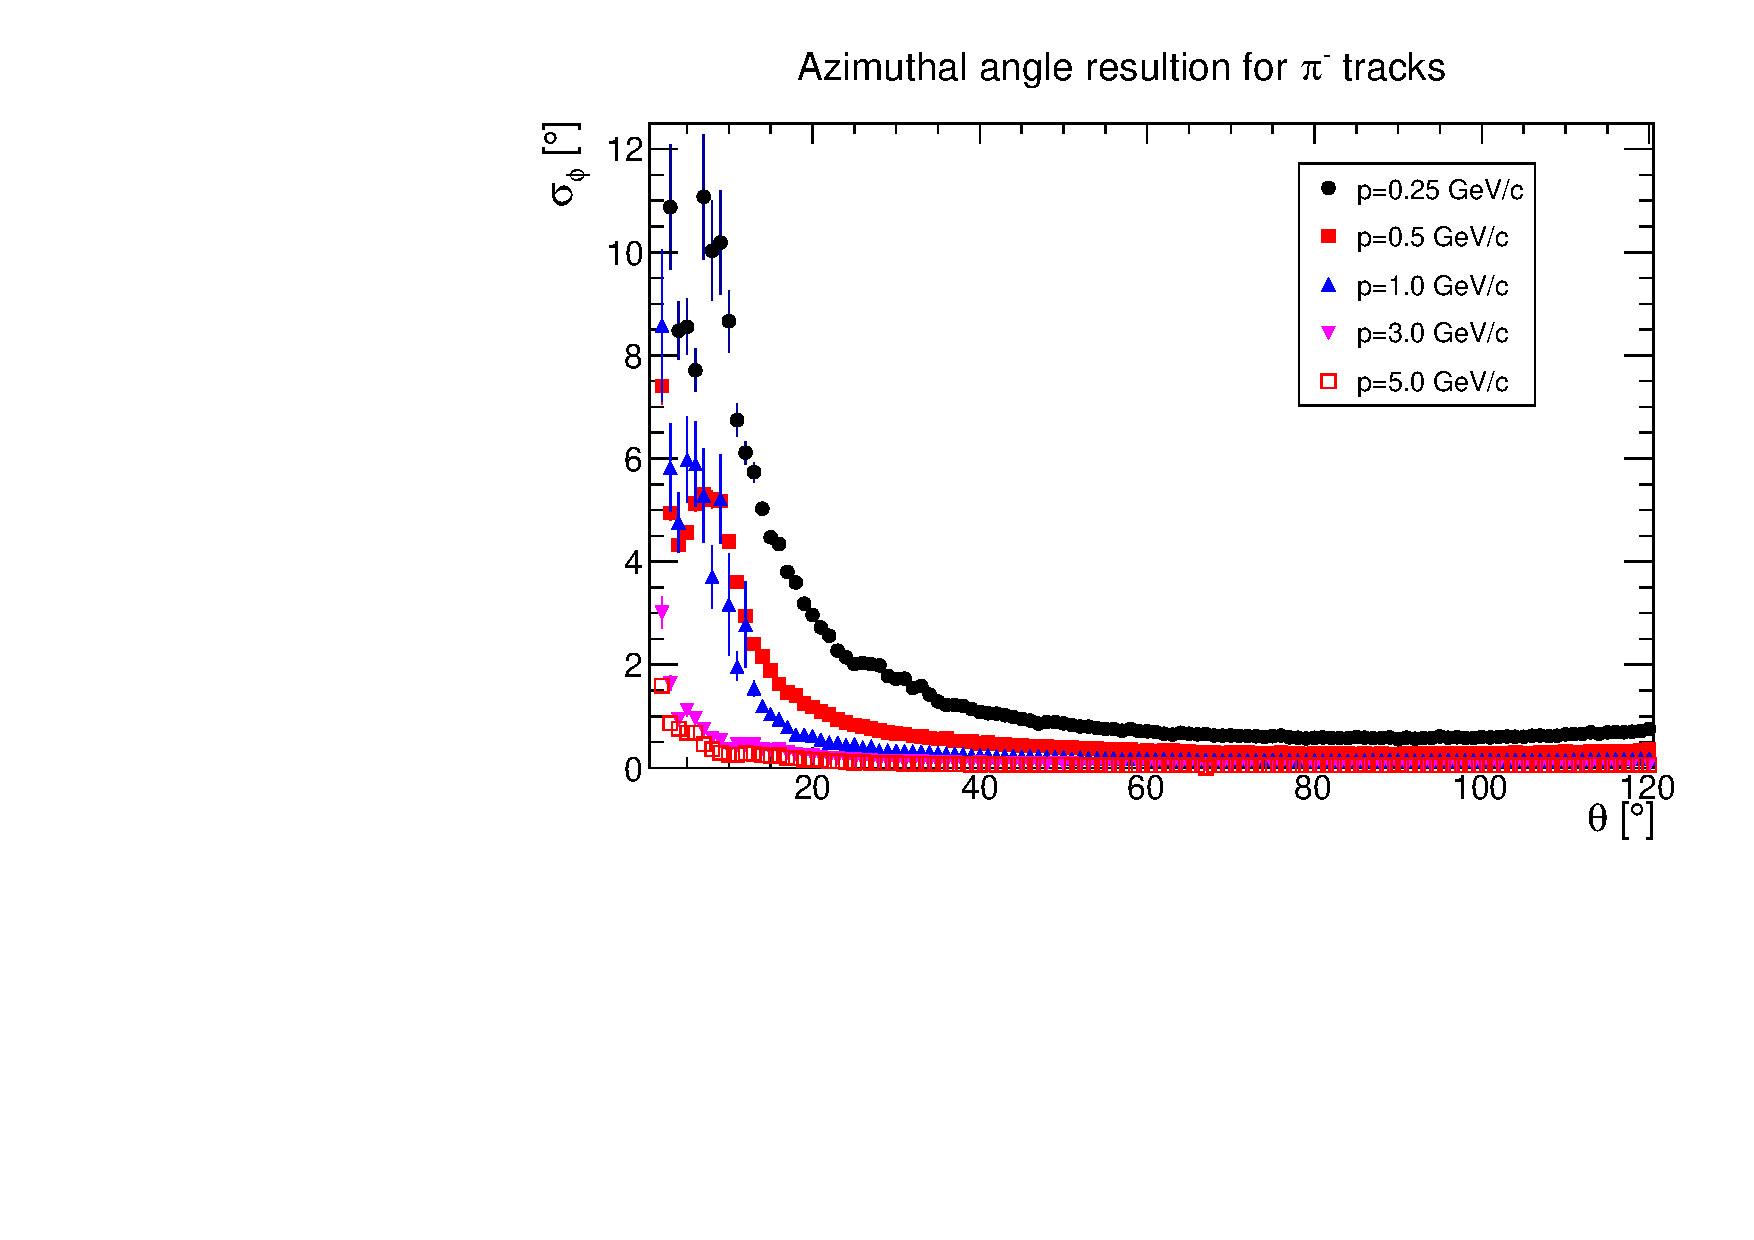
\includegraphics[width=0.45\textwidth]{figures/PionPhiResolution.pdf}
\caption{\label{fig:angle res} (Left) Polar angle resolution for $\pi^-$ tracks.
(Right) Azimuthal angle resolution for $\pi^-$ tracks.
The resolutions are plotted as a function of the polar angle, $\theta$.}
\end{center}
\end{figure}


\subsection{Vertex resolution}

The thin windows of the cryogenic target and the exit window of the target
vacuum chamber provide a means to estimate the 
vertex resolution of the tracking system.  Pairs of tracks from empty target runs are used to reconstruct these windows as illustrated in 
Fig.~\ref{fig:z-vertex}. The distance of closest approach between two tracks, $d$, was required to be less than 1~cm. The vertex position 
is at the mid-point of the line segment (of length $d$) defined by the points of closest approach for each track.
The estimated $z$-position resolution is 3~mm.

\begin{figure}[tbp]
\begin{center}
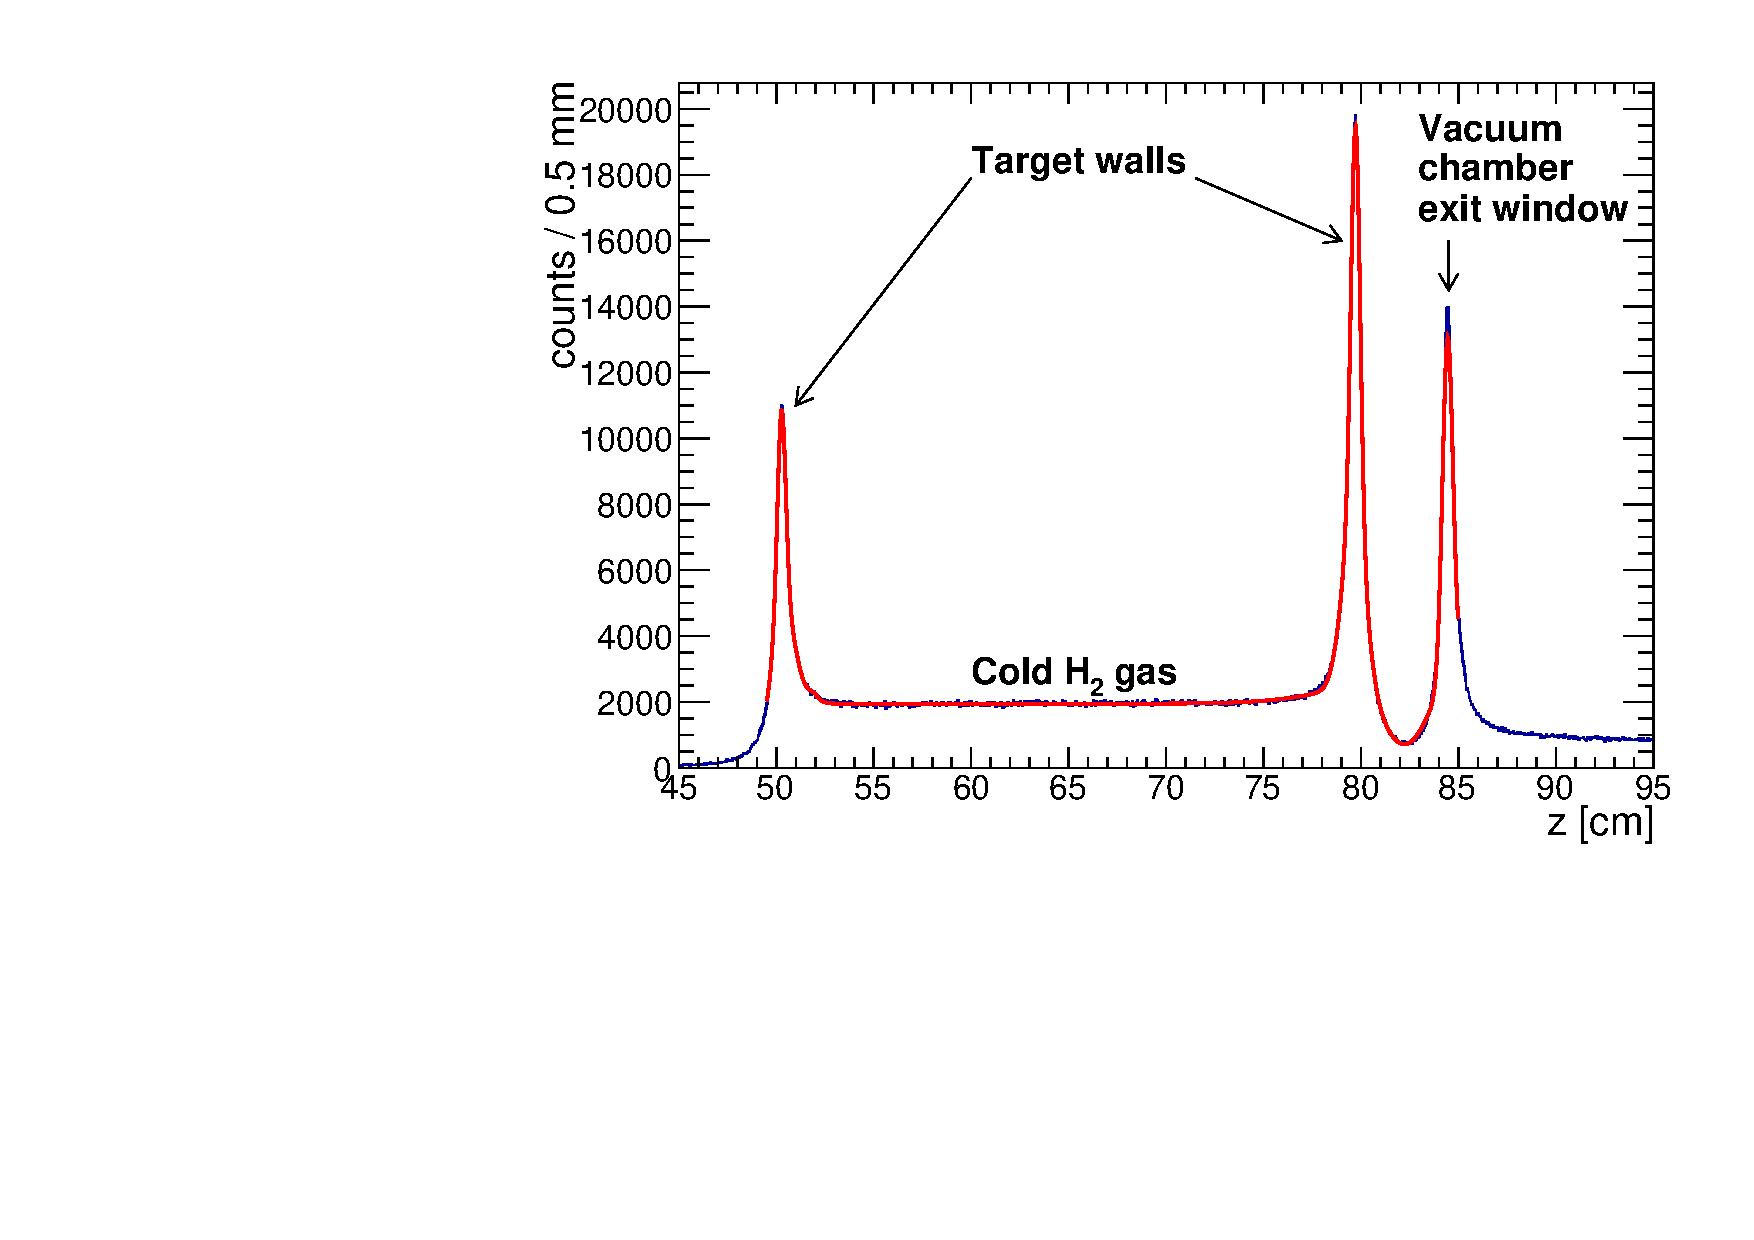
\includegraphics[width=0.7\textwidth]{figures/ZVertex.pdf}  
\caption{\label{fig:z-vertex} Reconstructed vertex positions within 1 cm radial
 distance with respect to the beam line for an empty target run.  The curve shows the result of a fit to the vertex distribution used to determine the vertex
resolution. 
}   
\end{center}  
\end{figure}

